\documentclass{article}
\usepackage[utf8]{inputenc}
\usepackage[usenames,dvipsnames,pdftex]{xcolor}
\usepackage{fullpage}
\usepackage[upright]{fourier}
\usepackage{tkz-graph}
\usetikzlibrary{arrows}
\thispagestyle{empty}
\begin{document}
\begin{center}
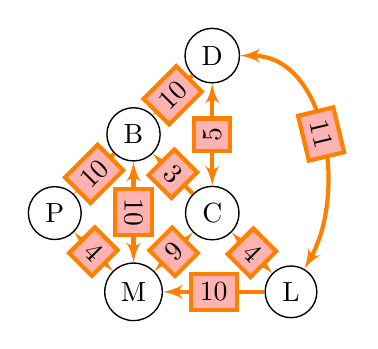
\begin{tikzpicture}[>=latex']
 \SetUpEdge[lw         = 1.5pt,
            color      = orange,
            labelcolor = red!30,
            labelstyle = {draw,sloped}]
  \tikzset{node distance = 5cm}
  \GraphInit[vstyle=Normal]
  \Vertex{P}
  \NOEA(P){B}
  \SOEA(P){M}
  \NOEA(B){D}
  \SOEA(B){C}
  \SOEA(C){L} 
  \tikzset{EdgeStyle/.style={->}}
  \Edge[label=$3$](C)(B)
  \Edge[label=$10$](D)(B)
  \Edge[label=$10$](L)(M)
  \Edge[label=$10$](B)(P)
  \tikzset{EdgeStyle/.style={<->}}
  \Edge[label=$4$](P)(M)
  \Edge[label=$9$](C)(M)
  \Edge[label=$4$](C)(L)
  \Edge[label=$5$](C)(D)
  \Edge[label=$10$](B)(M)
  \tikzset{EdgeStyle/.style={<->,relative=false,in=0,out=60}}
  \Edge[label=$11$](L)(D)
\end{tikzpicture}
\end{center}
\end{document}
% Author : Alain Matthes
% Encoding : UTF8
% Engine : PDFLaTeX
